\chapter[Uranium Enrichment Regression \newline Results and Discussion]{Uranium Enrichment Regression Results and Discussion} \label{uranium-enrichment}

Measuring uranium enrichment is difficult for a number of reasons. First, characteristic $^{235}$U gamma-rays are easily shielded. Second, restriction may be placed on inspectors performing measurements for treaty verification. Inspectors can face two major restrictions: a limited amount of time to measure data and the requirement for an information barrier. An information barrier is anything that restricts the inspector from measuring information outside of their specific target. For example, if an inspector measured the gamma-ray spectrum of an object using a high-resolution HPGe detector, they could extract information about the process used to process used to bred and enrich the material. This information could be a state secret, and thus would need to be protected with some barrier. The low-resolution inherent to NaI(Tl) is an information barrier for treaty verification measurements. An addition information barrier is an ANN which is trained to only extract enrichment information. 

This chapter demonstrates a validation demonstration applying \verb|annsa| to automated uranium enrichment measurements using NaI(Tl). In this chapter we discuss how we used MCNP and GADRAS-DRF to create spectral templates for training dataset simulation with \verb|annsa|. We also train and benchmark ANNs on simulated and measured enriched uranium spectra measured at the Nevada National Security Site and as part of a IAEA training exercise.


\section{Uranium Enrichment Measurement Background}

Verifying the enrichment of HEU through passive nondestructive analysis is important for nuclear safeguards applications and homeland security tasks. Passive nondestructive analysis, such as gamma-ray spectroscopy, is preferred to more accurate destructive methods due to its ability to operate quickly, preserve forensic evidence, and allow for remote measurements. The enriched uranium gamma-ray signatures visible in low-resolution detectors come from the decay of $^{238}$U, $^{235}$U, $^{232}$U, and the daughters of these isotopes. Figure \ref{fig:enriched_u_peaks_displayed} shows an example of a 27\% enriched uranium spectrum that displays $^{238}$U and $^{235}$U photopeaks. In low-resolution detectors, The primary photopeaks from $^{235}$U are at 144 keV, 163 keV, and 186 keV. The $^{238}$U daughter $^{234m}$Pa produces two main photopeaks at 766 keV and 1001 keV. $^{232}$U, only present in reprocessed uranium, produces a photopeak at 2.6 MeV from its $^{208}$Tl daughter.

\begin{figure}[H]
	\centering
	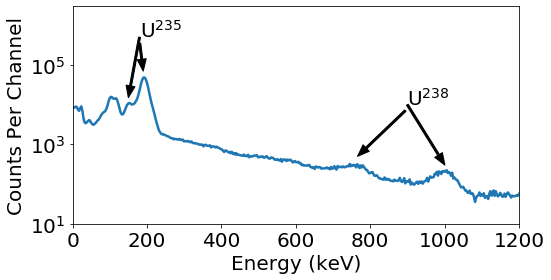
\includegraphics[width=0.8\linewidth]{images/enriched_u_peaks_displayed}
	\caption{27\% enriched uranium spectrum measured with a NaI(Tl) detector.}.
	\label{fig:enriched_u_peaks_displayed}
\end{figure}

Traditionally, the enrichment meter method is used to measure uranium enrichment in NaI(Tl) spectra \cite{Reilly1970}. This, and all enrichment measurement methods based on gamma-ray spectroscopy, only measures the enrichment of an object's surface to a depth of 0.26 cm and 0.74 cm for uranium metal and U$_{3}$O$_{8}$ powder, respectively \cite{Pandas}. At these material depths, the attenuation properties of uranium removes 99.8\% of the 186 keV signal. The enrichment meter method method exploits the proportionality between the activity of the 186 keV photon and the enrichment of $^{235}$U. The enrichment meter method works by finding calibration constants that relate counts in two ROIs,
%
\begin{align} \label{eq:enrichment_meter_principle}
E &= A  C_{ROI1} + B C_{ROI2} 
\intertext{where}
C_{ROI1} &= \text{counts in ROI1 [\# counts]} \nonumber \\
C_{ROI2} &= \text{counts in ROI2 [\# counts]} \nonumber \\
A &= \text{calibration constant} \nonumber \\
B &= \text{calibration constant,} \nonumber
\end{align}
%
to the measured material's enrichment. These ROIs are placed around the 186 keV peak and in the background region to the right of the peak. Finding these constants requires measuring two different uranium enrichment standards in the same configuration (shielding, scattering environment, source-detector distance). Once these calibration constants are measured, they can only be used in the same configuration as the reference standards. It is possible to extend this method to other shielding configurations, but this introduces a risk of adding systematic errors. An automated version of this method called NaIGEM (NaI(Tl) Gamma Enrichment Measurements) is included in the HM-5 instrument used by the IAEA \cite{MORTREAU2004}. Enrichment measurements of uranium without contaminants using low-resolution detectors can achieve 1\% precision for arbitrary enrichments while  contamination by minor uranium isotopes have a biasing effect of 5-10\% \cite{SPRINKLE1997}. Measurements of materials with unknown enrichment, shielding, and geometry are typically performed with high resolution HPGe detectors using the Multi-Group Analysis for Uranium (MGAU) software \cite{MGAU1994}. Using a NaI(Tl) detector to measure the enrichment of an item without knowing these parameters is inherently challenging due to the low-resolution of NaI(Tl). By training ANNs with a dataset of simulated enriched uranium spectra, it may be possible to use this material to perform uranium enrichment measurements.


% "Generally, low resolution measurements of 'clean' uranium can be made to 1\% precision over nearly the entire range of uranium enrichment. Measurements in both Europe and the Former Soviet Union have observed bias effects of 5-10\% in low-resolution measurements caused by minor isotopes of uranium. This level of bias has been deemed unacceptable, causing some inspectors to resort to more expensive, time-consuming alternatives like mass spectrometry or liquid-nitrogen-cooler high-resolution detectors. As the international safeguards community attempts to inspect more facilities with less resources, these alternatives become highly undesirable. The minor isotopes come from the use of uranium recycled from reactors being used as feed in the enrichment plants. Daughters of $^{232}$U or $^{236}$U include the thorium decay chain which emits a 238.6-keV gamma ray from $^{212}$Pb. This gamma ray falls in the ROI used to estimate the Compton continuum under the 186-keV gamma ray. In addition, the multitude of high-energy gamma rays from the daughters of $^{232}$U change the shape of the Compton continuum that lies under the desired 186-keV peak. Just to make the entire issue more challenging, the level of this interference varies widely among the samples generally offered to the inspector, causing unpredictable, wide variations in the bias effects" \cite{SPRINKLE1997}

% Accuracies of +/- 10\% are expected for quick checks of high enriched material while accuracies of +/- 1\% are expected to verify mass spectroscopy measurments \cite{Kull1974}.

% Changes in background in the facility may affect performance. Studies done measuring uranium enrichment in marine environments have shown that background radiation is important and that existing methods  \cite{Hofstetter2008}.


\section{Problem Description and Training Dataset Overview}

To investigate how well a machine learning algorithm can learn to perform uranium enrichment measurements, machine learning architectures found in Chapter \ref{ChapterMachineLearningModelsExplored} were trained using a dataset of simulated enriched uranium spectra. 



% u232 production reactions from uranium species https://www.pnnl.gov/main/publications/external/technical_reports/PNNL-12075.pdf

% FRAM application to U and Pu isotopics https://www.lanl.gov/orgs/n/n1/appnotes/LA-14018-M.pdf

\subsection{Training Outline}

Simple and complete model architectures discussed in Sections \ref{table:hyperparameter_opt_parameters_DNN} and \ref{table:hyperparameter_opt_parameters_CNN} were trained using dataset of 10$^{5}$ simulated uranium spectra. Model architectures were modified to perform regression. Modifications include changing: the number of output nodes to one, their output function to a sigmoid, and their main cost function to mean squared error. Typically the sigmoid output function is used in the context of logistic regression. In our case the regression targets, percent $^{235}$U enrichment, exist on [0,1], allowing use of the sigmoid output function. Using this function, we interpret each ANN's output as an enrichment value on [0,1] instead of a list of isotope posterior probabilities. Pretrained simple and complete DAE and CAE models from Section \ref{section_autoencoder_archetectures} were also fine-tuned using the simulated uranium dataset. Each model was trained using 5-folds cross validation. For each test dataset in this chapter, uranium enrichment predictions from each trained model were averaged to reduce the prediction's variance. This process is illustrated in Figure \ref{fig:uenrich_training_outline}.

\begin{figure}[H]
	\centering
	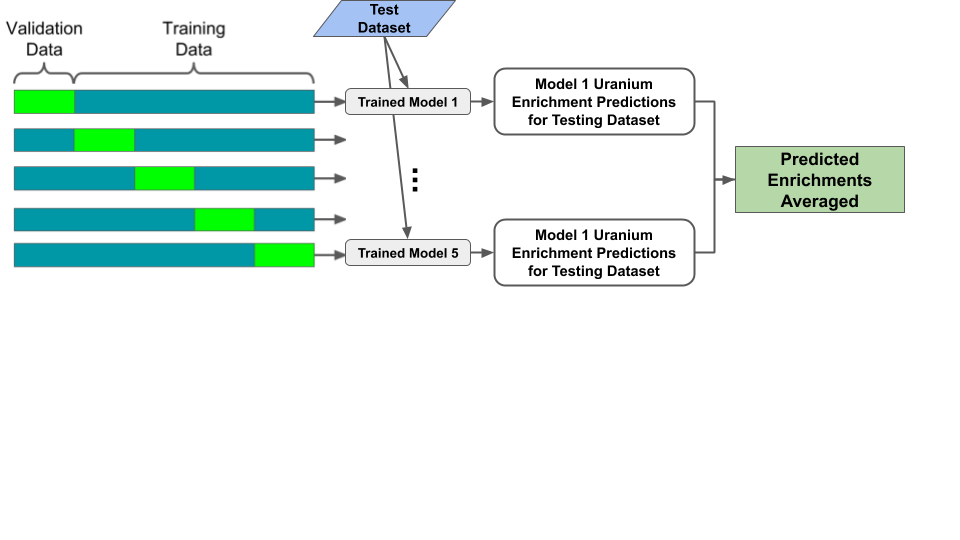
\includegraphics[trim=0 250 40 0,clip,width=1.0\linewidth]{images/uenrich_training_outline}
	\caption{Training and prediction averaging.}
	\label{fig:uenrich_training_outline}
\end{figure}

\subsection{Training Dataset Details}

A coupled MCNP (Monte Carlo N-Particle Transport Code) and GADRAS-DRF code was used to simulate the spectrum from each uranium isotope uniformly distributed in a solid uranium sphere of radius 5.5 cm. MCNP simulation was used to calculate the physics due to self attenuation in the uranium and GADRAS-DRF was used to model the gamma-ray spectrum from this source in a 2'' x 2'' NaI(Tl) detector. The universe in the MCNP simulation, shown in Figure \ref{fig:mcnp_diagram}, was empty except for a 19 cm concrete block fixed at 180 cm from the origin, a 5.5 cm radius sphere of bare uranium fixed at the origin, and a bare 2'' x 2'' NaI(Tl) cylinder located between them. The concrete block was added to incorporate backscatter radiation in the MCNP simulation. A total of 10$^{8}$ particles were simulated for each configuration.

\begin{figure}[H]
	\centering
    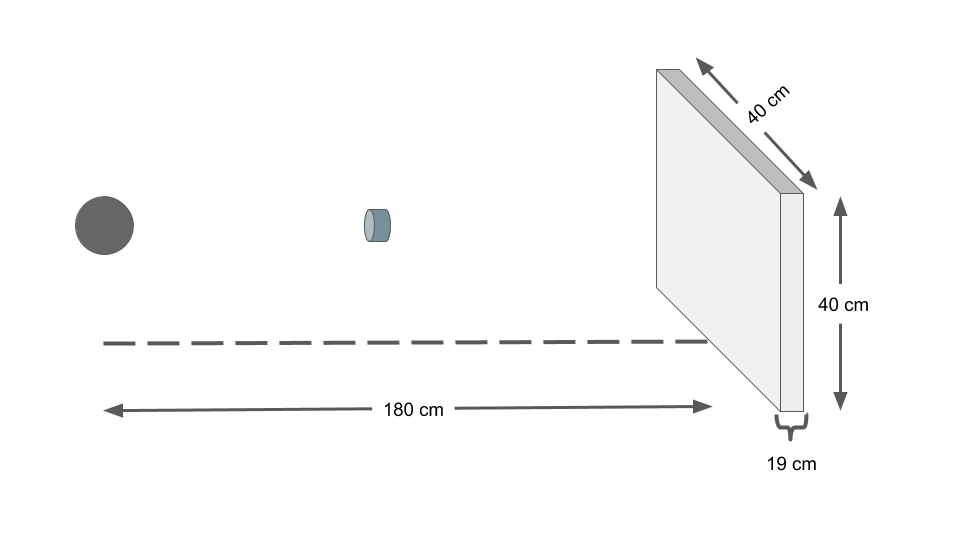
\includegraphics[trim=50 50 50 50,clip,width=0.99\linewidth]{images/mcnp_diagram.png}
	\caption{Diagram of MCNP simulation (not to scale).}
	\label{fig:mcnp_diagram}
\end{figure}

The software package RadSrc was used to generate specific gamma-ray intensities for the $^{235}$U, $^{238}$U, and $^{232}$U templates \cite{Hiller2007}. RadSrc, developed at Lawrence Livermore National Laboratory, uses the Bateman equations to calculate daughter in-growth and their respective specific gamma-ray intensities. Isotopes in enriched uranium reach secular equilibrium in about six months. To account for this, RadSrc was used to find specific gamma-ray intensities for 50 year old uranium isotopes and their ingrown daughters. The specific activities for each isotope are found in Table \ref{table:specific_activities_radsrc}.

\begin{table}[H]
\centering
\caption{Specific activities for 50 year old uranium isotopes and their ingrown daughters.}
\label{table:specific_activities_radsrc}
\begin{tabular}{lr}
\hline
\textbf{Isotope} & \textbf{Specific Gamma-ray Activity [$\frac{\gamma}{g s}$]} \\ \hline
$^{232}$U & 1.20 x 10$^{12}$ \\ 
$^{235}$U & 2.07 x 10$^{5}$ \\
$^{238}$U & 3.80 x 10$^{3}$ \\ \hline
\end{tabular}
\end{table}

$^{235}$U and $^{238}$U templates were combined in weighted combinations to create spectra of desired enrichments using the process described previously in Equation \ref{eq:template_sampling}. To account for factors that change the $^{232}$U content, each sample that included $^{232}$U used a mass fraction uniformly chosen between 4 x 10$^{-9}$ and 2 x 10$^{-8}$ \cite{Peurrung2019}. To account for clean uranium, the probability that a spectrum was simulated with $^{232}$U was 0.5. Complete simulation parameters for the coupled MCNP and GADRAS-DRF approach are shown in Table \ref{table:hyperparameter_dataset_full_parameters_enrichment}.

\begin{table}[H]
\centering
\caption{Range of parameters used for the uranium enrichment dataset.}
\label{table:hyperparameter_dataset_full_parameters_enrichment}
\begin{tabular}{lll}
\hline
\textbf{Simulation Parameter} & \textbf{Range} & \textbf{Sampling} \\ \hline
Source-Detector Distance [cm] & 25, 50, 100, 150, 200 & Uniform \\ % \hline
FWHM 662 keV [s] & 6.5, 7.0, 7.5 & N/A \\ % \hline
Shielding (\% 200 keV Attenuated) & 0\%, 20\%, 40\%, 60\% & Uniform \\ % \hline
Integration Time [s] & 60 - 3600 & Log-Uniform \\ % \hline
Calibration Offset [channels] & -10 - 10 & Uniform \\ % \hline
Calibration Gain & 0.8 - 1.2 & Uniform \\ % \hline
$^{235}$U Enrichment [\%] & 0 - 100 & Uniform \\ % \hline
Background Counts per Second & 170 - 230 & Uniform \\ % \hline
Signal to Background Ratio & 1.0 - 4.0 & Log-Uniform \\ \hline
\end{tabular}
\end{table}


\section{Results - Simulated Data}

These sections describe how each trained model performs when predicting the uranium enrichment of simulated spectra. To investigate performance, spectra were simulated with enrichments of 3\%, 25\%, 50\%, 75\%, and 93\% in different conditions. To observe each ANN's enrichment prediction variance, 10 spectra were simulated for each enrichment value. Each ANN's mean and variance when identifying all spectra at each enrichment value was recorded. Each ANN used the model averaging technique shown in Figure \ref{fig:uenrich_training_outline}. Default simulation parameters are shown in Table \ref{table:default_sim_params_uranium}. Changes to these defaults are indicated for each generalization experiment.

\begin{table}[H]
\centering
\caption{Default parameters used for all generalization datasets.}
\label{table:default_sim_params_uranium}
\begin{tabular}{lr}
\hline
\textbf{Simulation Parameter} &  \textbf{Value} \\ \hline
Source-Detector Distance [cm] & 50.0\\ 
FWHM 662 keV [s] & 7.0\\
Shielding (\% 200 keV Attenuated) & 0\% \\ 
Integration Time [s] & 600.0 \\ 
Calibration - Offset (channels) & 0.0 \\ 
Calibration - Gain & 1.0 \\ 
Signal to Background Ratio & 3.0 \\ 
Background Counts Per Second & 200.0 \\ \hline
\end{tabular}
\end{table}

\subsection{Effect of Shielding on Enrichment Prediction}

To test each model's ability to measure uranium enrichment when the uranium source is shielded, enriched uranium spectra were simulated with various thicknesses of shielding. The effect of each shielding thickness is shown in Figure \ref{fig:simulated_uranium_shielding}. The predicted enrichments from each model on these cases are shown in Figure \ref{fig:simuranium-shielding}. In general for each case, the complete networks outperform the simple networks by predicting enrichments closer to the simulated value. This indicates that the reduced capacity of the simple networks is insufficient to properly perform uranium enrichment measurements using the provided dataset. At 93\% enrichment each model underestimates the enrichment.

\begin{figure}[H]
	\centering
	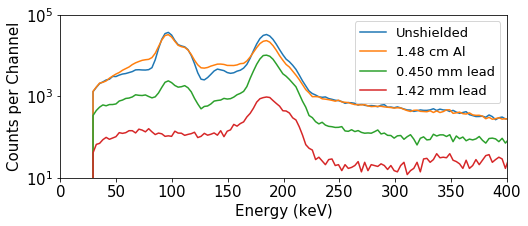
\includegraphics[width=0.8\linewidth]{images/simulated_uranium_shielding.png}
	\caption{Simulated 93\% enriched uranium spectra various amounts of shielding.}
	\label{fig:simulated_uranium_shielding}
\end{figure}

\begin{figure}[H]
     \centering
     \begin{subfigure}[b]{0.49\textwidth}
         \centering
         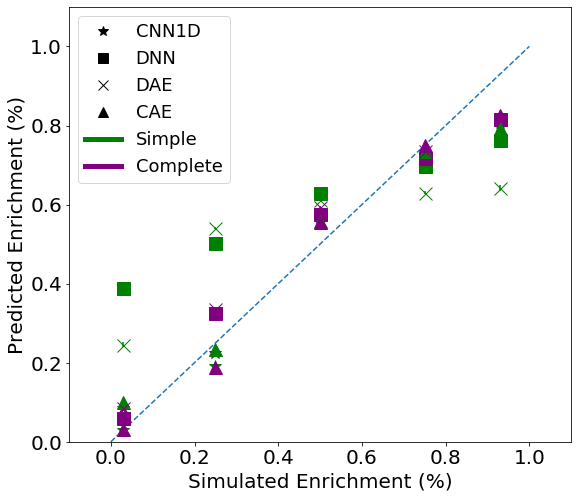
\includegraphics[width=\textwidth]{images/simuranium-noshield.png}
         \caption{Unshielded.}
         \label{fig:simuranium-noshield}
     \end{subfigure}
     \hfill
     \begin{subfigure}[b]{0.49\textwidth}
         \centering
         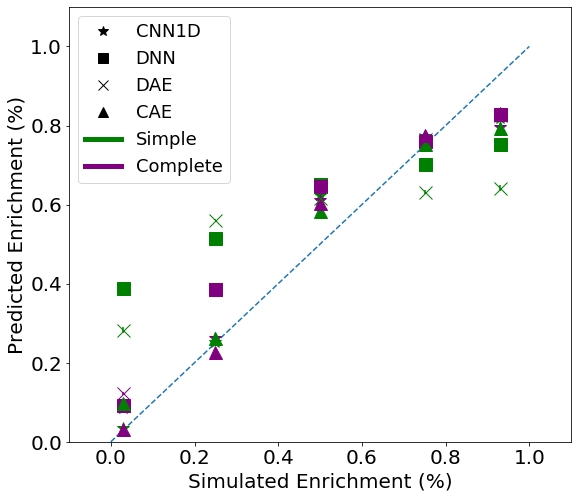
\includegraphics[width=\textwidth]{images/simuranium-lightal.png}
         \caption{1.48 cm aluminum.}
         \label{fig:simuranium-lightal}
     \end{subfigure}

     \begin{subfigure}[b]{0.49\textwidth}
         \centering
         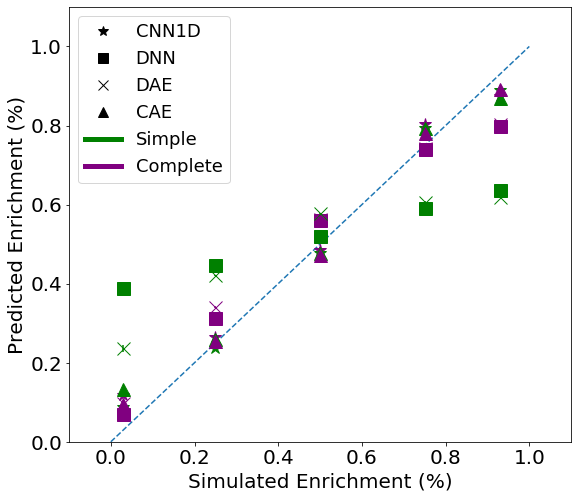
\includegraphics[width=\textwidth]{images/simuranium-mediumlead.png}
         \caption{0.450 mm lead.}
         \label{fig:simuranium-mediumlead}
     \end{subfigure}
     \hfill
     \begin{subfigure}[b]{0.49\textwidth}
         \centering
         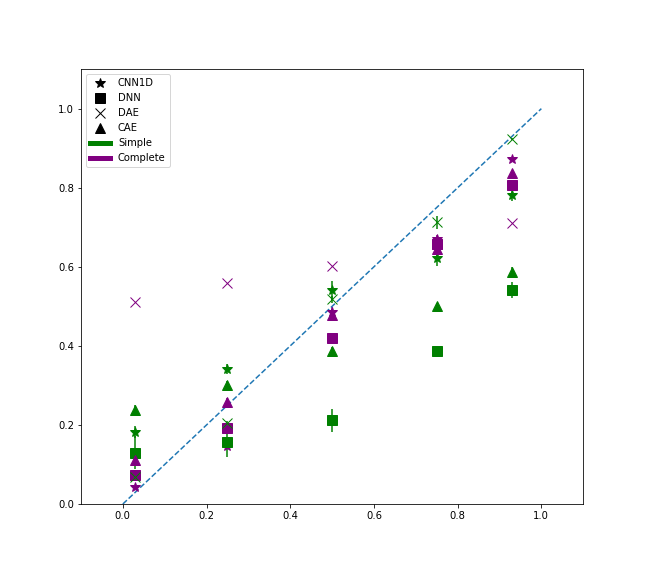
\includegraphics[width=\textwidth]{images/simuranium-heavylead.png}
         \caption{1.42 mm lead.}
         \label{fig:simuranium-heavylead}
     \end{subfigure}
        \caption{Each model's prediction for the uranium enrichment of spectra simulated with different shielding thicknesses. Shielding conditions are indicated below each figure.}
        \label{fig:simuranium-shielding}
\end{figure}

In all cases except with 1.42 mm of lead shielding, simple networks overestimate the enrichment at and below 50\%. The simple models also underestimate the enrichment at values over 50\%. This reinforces the conclusion that the simple network has too little capacity to fit the data. Because the range of enrichments in the training data are uniformly distributed from 0 - 100\%, the naive method to minimize the cost function is to predict enrichments near 50\%. The complete models were 
within 20\% of the true value in all cases except with 1.42 mm of lead shielding. This shows that complete models are only affected by relatively large amounts of shielding.


\subsection{Effect of Calibration on Enrichment Prediction} \label{section_uranium_sim_cal}

In this section we test each model's ability to measure uranium enrichment in spectra with various relative calibration gains. The predict enrichments from each model on these cases are shown in Figure \ref{fig:simuranium-cal}. Model performance at relative gains of 0.9 and 1.1 are similar to the reference gain case, shown in Figure \ref{fig:simuranium-noshield}.

\begin{figure}[H]
	\centering
	\begin{subfigure}[b]{0.49\textwidth}
		\centering
		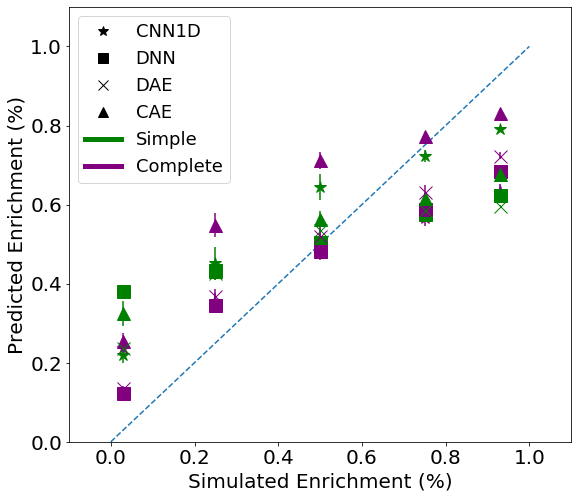
\includegraphics[width=\textwidth]{images/simuranium-cal08.png}
		\caption{0.8}
		\label{fig:simuranium-cal08}
	\end{subfigure}
	\hfill
	\begin{subfigure}[b]{0.49\textwidth}
		\centering
		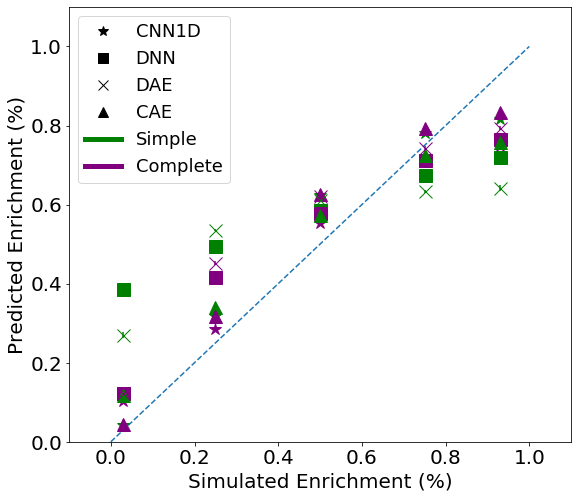
\includegraphics[width=\textwidth]{images/simuranium-cal09.png}
		\caption{0.9}
		\label{fig:simuranium-cal09}
	\end{subfigure}
	
	\begin{subfigure}[b]{0.49\textwidth}
		\centering
		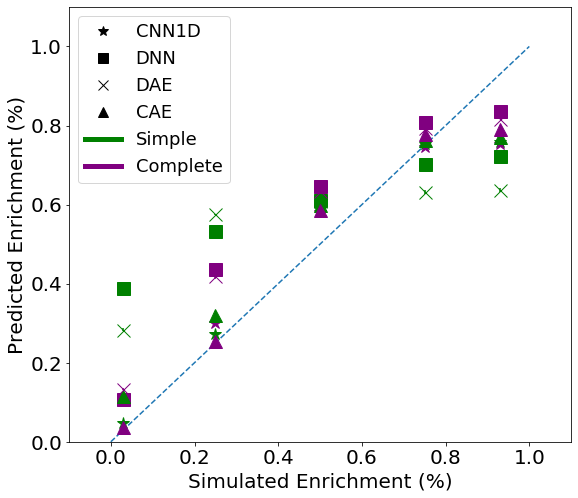
\includegraphics[width=\textwidth]{images/simuranium-cal11.png}
		\caption{1.1}
		\label{fig:simuranium-cal11}
	\end{subfigure}
	\hfill
	\begin{subfigure}[b]{0.49\textwidth}
		\centering
		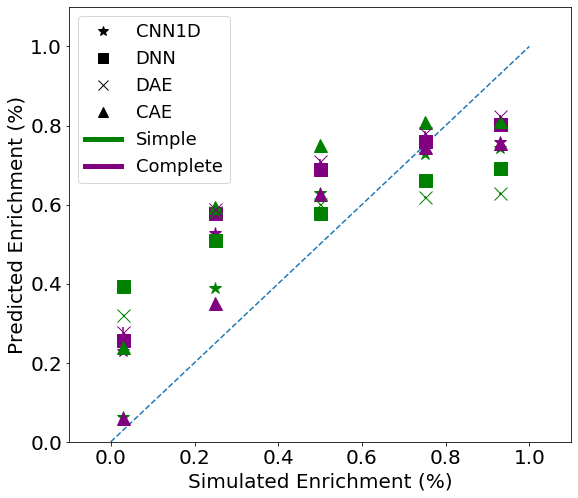
\includegraphics[width=\textwidth]{images/simuranium-cal12.png}
		\caption{1.2}
		\label{fig:simuranium-cal12}
	\end{subfigure}
	\caption{Each model's prediction for the uranium enrichment of simulated spectra calibrated with  different gain settings. The magnitude of the applied relative gain shift are shown below each figure.}
	\label{fig:simuranium-cal}
\end{figure}


At the extreme relative gain shifts of 0.8 and 1.2 each ANN's performance visibly changes compared to the reference gain. These shifts represent large deviations in normal NaI(Tl) operating temperature or a significantly miscalibrated detector. At a relative gain shift of 0.8, the dense models are not visibly impacted compared to the reference gain case when measuring uranium with enrichments below 75\%. 

At a gain shift of 1.2 each ANN overestimates enrichment for enrichments at and below 50\%. The complete CAE and simple CNN are the most accurate when predicting enrichment values at and below 25\%. Because the 1.2 relative shift moves the 766 keV and 1001 keV $^{238}$U peaks into regions of little importance for the spectra without gain shift, seen in Figure \ref{fig:simulated_uranium_calibration_10pct}, these peaks are ignored and the enrichment is overestimated.


\begin{figure}[H]
	\centering
	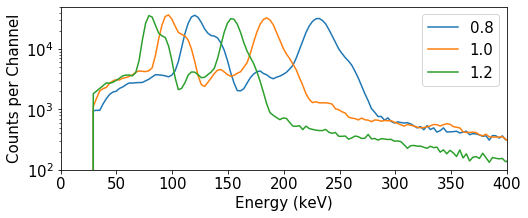
\includegraphics[width=0.8\linewidth]{images/simulated_uranium_calibration.png}
	\caption{Simulated 93\% enriched uranium spectra with three different relative gain settings. Energy calibration shown is based on the 1.0 relative gain setting.}
	\label{fig:simulated_uranium_calibration_93pct}
\end{figure}

\begin{figure}[H]
	\centering
	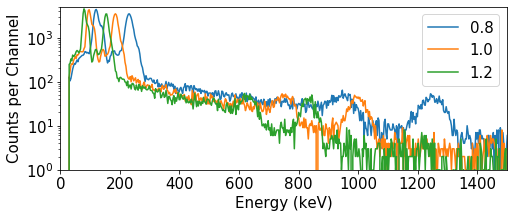
\includegraphics[width=0.8\linewidth]{images/simulated_uranium_calibration_1500kev.png}
	\caption{Simulated 10\% enriched uranium spectra with three different relative gain settings. Energy calibration shown is based on the 1.0 relative gain setting.}
	\label{fig:simulated_uranium_calibration_10pct}
\end{figure}

\section{Results - Measured Spectra}

To quantify performance in real gamma-ray spectra, material with different uranium enrichments were measured with a variety of NaI(Tl) detectors. Objects measured include a 13 kg 93\% enriched uranium metal sphere \cite{Rothe1997} measured at the Nevada National Security Site and three U$_{3}$O$_{8}$ samples measured as part of an IAEA training exercises \cite{jacobstinnett_u3o8}. Shielding, source-detector distance, radiation background, and scattering environments were not recorded for the training exercise. The U$_{3}$O$_{8}$ spectra were measured with energies below 1.3 MeV. Energies above this threshold do not include information about the object's enrichment, so removing it will have negligible effect on the ANN predictions. In addition to this, each detector used to measure the U$_{3}$O$_{8}$ spectra had a unique calibration. We manually recalibrated each spectrum using gain and offset correction to match each 186 keV and 1001 keV photopeak. These recalibrated spectra are shown in Figure \ref{fig:measured_uranium_plots}.

\begin{table}[H]
\centering
\caption{Uranium sample description.}
\label{table:uranium_sample_description}
\begin{tabular}{cccc}
\hline
Enrichment & $^{235}$U Mass (g) & Material & Live Time (s)   \\ \hline
93.1\% & 13,000 & U Metal & 300 \\
91.4\% & 903 & U$_{3}$O$_{8}$ &  226\\
27.1\%  & 264 & U$_{3}$O$_{8}$ & 344 \\ 
0.7\% & - & U$_{3}$O$_{8}$ & 97.4 \\ \hline
\end{tabular}
\end{table}

\begin{figure}[H]
	\centering
	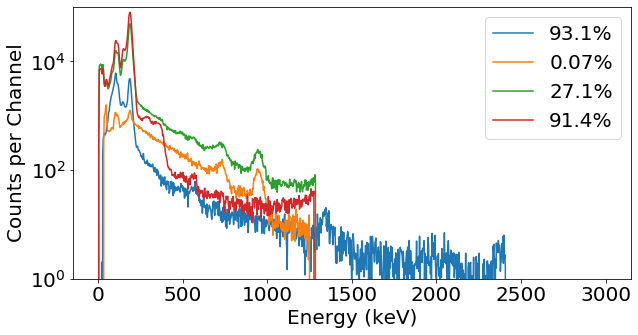
\includegraphics[width=0.8\linewidth]{images/measured_uranium_plots.png}
	\caption{Enriched uranium spectra recalibrated to the 186 keV and 1001 keV photopeaks.}
	\label{fig:measured_uranium_plots}
\end{figure}

Figure \ref{fig:measured_uranium} shows the predicted enrichment's mean and variance for each model and measured spectrum. Similar to the simulated spectra, the simple architectures underestimate enrichments over 50\% and overestimate enrichments under 50\%. Each network's prediction variance was not visible. In general, the complete architectures were more accurate than the simple architectures. 

\begin{figure}[H]
	\centering
	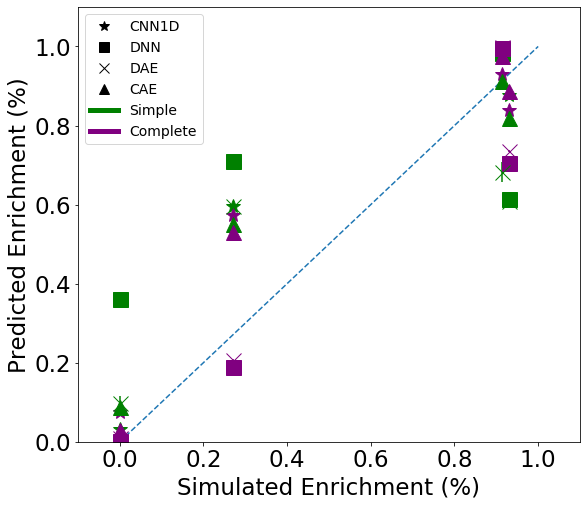
\includegraphics[width=0.8\linewidth]{images/measured_uranium.png}
	\caption{Each model's predicted uranium enrichment for measured uranium spectra.}
	\label{fig:measured_uranium}
\end{figure}

At 27.1\% enrichment, most ANNs overestimate the enrichment by at least 13 points. The complete dense models more accurately predict enrichment values for the 27.1\% enriched uranium spectrum. Spectra with lower enrichment include a continuum-like signal from an effect called bremsstrahlung. Bremsstrahlung (German for ``breaking radiation'') is produces when charged particles accelerate in the electric field of a heavy nucleus. In enriched uranium, bremsstrahlung is produced from the 2.3 MeV beta particle that is associated with the decay of $^{234m}$Pa, a $^{238}$U daughter. Convolutional models extract features based on their 16 channel filter kernel lengths. Without the bremsstrahlung signal in the training dataset, convolutional models have learned feature extraction techniques that cannot work when the bremsstrahlung signal is present in low-enriched data. Dense models are forced to extract features in patches of 16 channels, so they can more easily ignore the bremsstrahlung continuum and use the $^{235}$U and $^{238}$U photopeaks for enrichment prediction. 


To investigate how changing calibration effects each algorithm, the spectra from Figure \ref{fig:measured_uranium_plots} were recalibrated with the same gain settings explored in Section \ref{section_uranium_sim_cal}. Each ANN's enrichment prediction for these spectra is shown in Figure \ref{fig:realuranium-cal}.

\begin{figure}[H]
	\centering
	\begin{subfigure}[b]{0.49\textwidth}
		\centering
		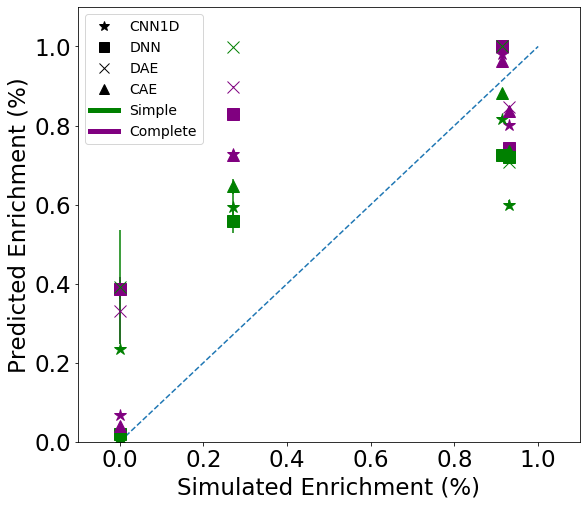
\includegraphics[width=\textwidth]{images/measured_uranium_08.png}
		\caption{0.8}
		\label{fig:measured_uranium_08}
	\end{subfigure}
	\hfill
	\begin{subfigure}[b]{0.49\textwidth}
		\centering
		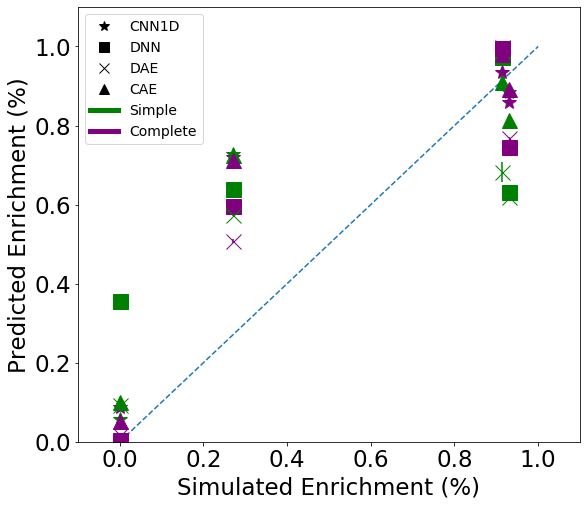
\includegraphics[width=\textwidth]{images/measured_uranium_09.png}
		\caption{0.9}
		\label{fig:measured_uranium_09}
	\end{subfigure}
	
	\begin{subfigure}[b]{0.49\textwidth}
		\centering
		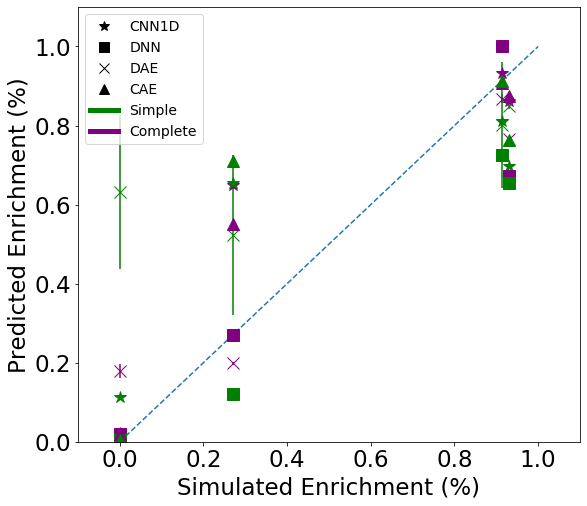
\includegraphics[width=\textwidth]{images/measured_uranium_11.png}
		\caption{1.1}
		\label{fig:measured_uranium_11}
	\end{subfigure}
	\hfill
	\begin{subfigure}[b]{0.49\textwidth}
		\centering
		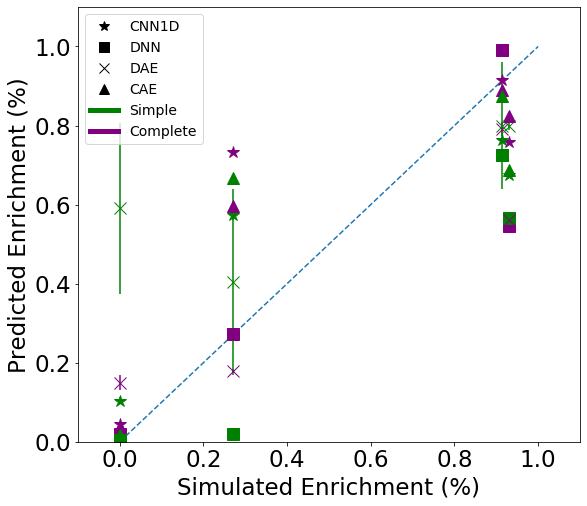
\includegraphics[width=\textwidth]{images/measured_uranium_12.png}
		\caption{1.2}
		\label{fig:measured_uranium_12}
	\end{subfigure}
	\caption{Each model's prediction for the uranium enrichment of measured spectra calibrated with  different gain settings. The magnitude of the applied relative gain shift are shown below each figure.}
	\label{fig:realuranium-cal}
\end{figure}

Similar to the simulated results, relative gain settings of 0.9 and 1.1 do not significantly impact enrichment quantification for most networks. The relative gain setting of 0.9 increases the dense model's enrichment prediction for the 27\% enriched spectrum. In general, models overestimate the enrichment of 0.1\% and 27\% enriched spectra using the relative gain setting of 0.8. In all gain settings, ANNs underestimate 93\% enriched uranium spectrum's enrichment.


\section{Discussion and Conclusion}

The ability to distinguish low ($<$20\% $^{235}$U )and high ($>$85\% $^{235}$U) enriched uranium is extremely important. Low enriched uranium requires significant processing for use in a nuclear weapon while high enriched uranium requires much less processing. The current implementation can roughly differentiate between low and high enriched uranium. For example, it is reasonable to assume a sample of material is below 15\% enrichment if the complete DAE predicts an enrichment below 15\%. Similarly, complete DAE predictions above 25\% can be assumed to be high enriched uranium. Predictions within this range require additional testing to more accurately quantify enrichment.

This chapter shows that complete architectures outperform the simple architectures when predicting uranium enrichment. The results also show that the complete architectures tailored to isotope classification can be extend to other problems in gamma-ray spectroscopy. The chapter also demonstrates that autoencoders trained to reconstruct spectra for isotope identification can be used to pretrain networks for other spectroscopic tasks. The dense pretraining was shown to perform particularly well on both simulated and measured enriched uranium spectra. Dense models show promise in uranium enrichment regression. This is because the feature extraction processes used by the convolution architectures are tuned to isotope identification. The convolutional models used convolutional filters with lengths of 16 channels. Uranium enrichment regression may require shorter convolution filter lengths to extract features from photopeaks below 200 keV.

International safeguards measurements require high precision measurements in ranges similar to those offered by the enrichment meter method. To expand our presented method for use in international safeguards, the accuracy needs to be improved and tested on additional enriched uranium spectra. Accuracy can be improved by expanding the training dataset to include additional facility measurement scenarios. For measurement in nuclear processing facilities, additional scattering scenarios that mimic heavy equipment and small uranium samples that cannot be assumed to be infinitely thick at 186 keV must be added. The $^{232}$U, $^{234}$U, $^{233}$U, $^{236}$U, and bremsstrahlung contribution can also be modeled more accurately, especially to use this method in higher-resolution detectors.


